\subsection{Final Iteration: Reinforcement Learning}
\subsubsection{About}
The final iteration builds on the work from the previous iteration to explore an alternative approach to PCG. The Genetic Algorithm succeeded in terms
of creating meaningful levels for MiniDungeons, but it highlighted a bottleneck regarding scalability and deployment. 

When considering a real world implementation, the GA approach proved too computationally slow to be used for runtime level generation. 
To generate a high-fitness level, the GA generator requires approximately 30 seconds of evolutionary search.
Such an implementation would create unacceptable load times in a commercial video game. In comparison, a trained reinforcement learning (RL) agent 
would be able to output a level in just a few milliseconds \cite{khalifa2020pcgrl} by shifting the long computation time from runtime to training time. 

For that reason, this iteration explores the use of reinforcement learning to achieve similar results as the GA approach. 

\subsubsection{Evaluation}
The evaluation of the RL iteration focused on two distinct metrics: 
\begin{enumerate}
    \item \textbf{Training Convergence:} How fast the agent learned to optimize its reward function.
    \item \textbf{Level Generation Speed:} The agent's ability to quickly generate a new dungeon level.
\end{enumerate}

\textbf{Test Design:}
The objective of this evaluation was to validate the hypothesis that a neural network could generate MiniDungeon levels significantly 
faster than the Genetic Algorithm, without a significant loss in level quality.
\begin{itemize}
    \item \textbf{Training Stability:} Monitor the mean episode reward and the simulation delta reward over time to ensure the generator agent was 
    actively learning rather than randomly placing tiles.
    \item \textbf{Generation Speed Benchmark:} Compare the time required to generate a single level using the trained RL agent 
    against the GA implementation.
\end{itemize}

\textbf{Test Methodology:}
The RL agent was trained using Proximal Policy Optimization (PPO) \cite{schulman2017proximalpolicyoptimizationalgorithms} via the 
Stable Baselines 3 library \cite{stable-baselines3}. The training process ran for 1.000.000 timesteps.
\begin{enumerate}
    \item \textbf{Training Analysis:} Tensorboard logs were recorded to track the agent's smoothed reward curve.
    \item \textbf{Speed Test:} A benchmark script was created to generate 1000 levels and then measure the total time and average level generation time.
    \item \textbf{Solvability Test:} Using the same benchmark script, following the creation of 1000 levels. Each level was played by the deterministic agent from Iteration 2
    and the ratio of solvable to unsolvable levels was recorded as well as the delta reward ($Agent Reward - Level Difficulty$).
\end{enumerate}

\textbf{Results:}
\begin{itemize}
    \item \textbf{Training Convergence:} As shown in Figure \ref{fig:rl_training_curve}, the agent's reward stabilized after approximately 
    650.000 timesteps, indicating successful learning of the dungeon rules.
    \item \textbf{Speed Comparison:} The RL agent achieved an average generation time of \textbf{0.125 seconds} per level. 
    This represents a 240\% speed increase over the GA baseline of 30 seconds, validating the main motivation for this iteration.
    \item \textbf{Solvability:} The trained agent achieved a solvability rate of 91.2\%. This is lower than the GA version 
    that guarantees solvability with its fitness function, although it is sufficient for a system that can regenerate invalid levels in milliseconds.
    Additionally, the agent achieved an average delta reward of 8.699, meaning the target difficulty wasn't always reached by the generator. 
\end{itemize}

\begin{figure}[htbp]
\centerline{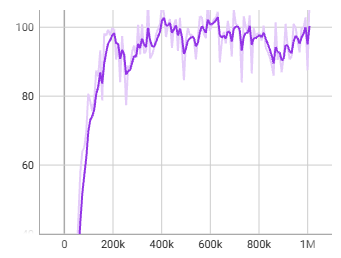
\includegraphics{assets/PPO40-v19-ep-rew-mean-sm.png}}
\caption{Mean Episodic Rewards for the RL level generator.}
\label{fig:rl_training_curve}
\end{figure}

\subsubsection{Reflections and decisions}
The results of this iteration confirm that Reinforcement Learning is a viable solution for runtime procedural content generation in MiniDungeons.

\textbf{Interpretation:}
The hypothesis regarding speed was strongly validated. The shift from evolutionary search to neural inference reduced 
generation time to negligible levels. However, the results also highlight the "Speed vs Reliability" trade-off presented by the different approaches. 
Unlike the GA, which evolves a level until it is perfect within the bounds of its fitness function, the RL agent attempts to construct a level 
in a single pass. This occasionally results in unsolvable map configurations (e.g. blocking the exit or too many forced monster encounters) 
or significantly easier than intended levels (e.g. the start and exit being directly adjacent).

\textbf{Decision:}
Given the high speed of the RL generator, the lower solvability rate is acceptable. In a real-world game loop, 
the system would simply discard unsolvable levels and generate a new one immediately without the player noticing a significant delay in load times. 
Therefore, the RL approach is deemed the superior version for a game requiring level generation at runtime, whereas the GA remains useful for scenarios
where levels are generated ahead of time, such as during a design process.

